\section{Patrons Non-retenus}
\subsection{Command dans le cas de la validation de commande}

\begin{figure}[!ht]
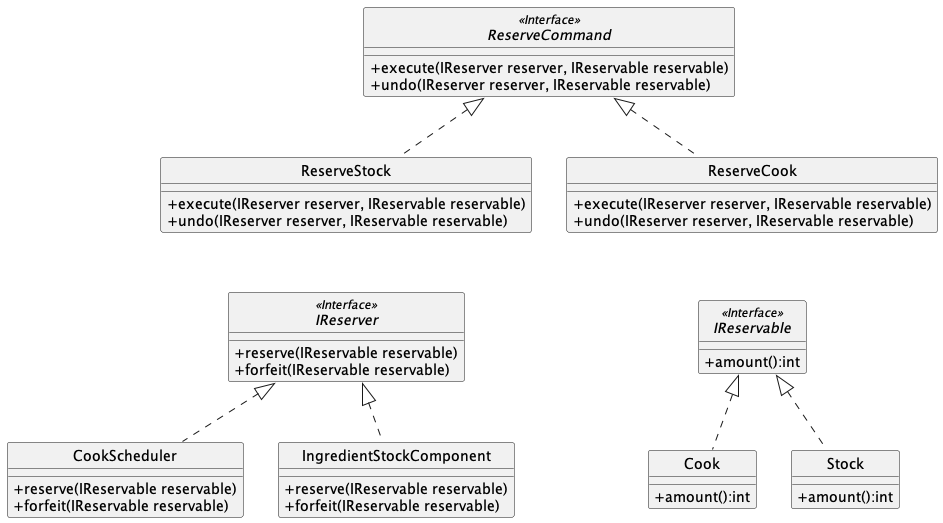
\includegraphics[width=0.8\textwidth]{commandPattern}
\centering
\caption{Diagramme de Classe d'étude préliminaire d'implémentation du patron de conception Command}
\label{uml:command}
\end{figure}

\paragraph{Command: } nous avons étudié l'implémentation du patron de conception command au niveau 
de la validation de commande par les clients. En effet, lors de la validation de commande, nous devons réserver
incrémentalement les ressources pour la préparation de la commande, avant de savoir si la commande va aboutir.
Ce patron de conception semblait donc judicieux, car il aurait permis de facilement annuler les réservations dans 
le cas ou la commande n'aboutit pas. Nous aurions également pu créer des MacroCommand composites qui représenteraient 
les commandes de cookies, ce qui faciliterais leur annulation.
Cependant, nous avons choisi de ne pas implémenter ce patron de conception, car il aurait impliqué de trop grandes modifications 
sur notre base de code sans entraîner de gains important étant donné que les fonctionnalités en question étaient déjà implémentées.

\subsection{State dans le cas de la gestion du status de la commande}

\begin{figure}[!ht]
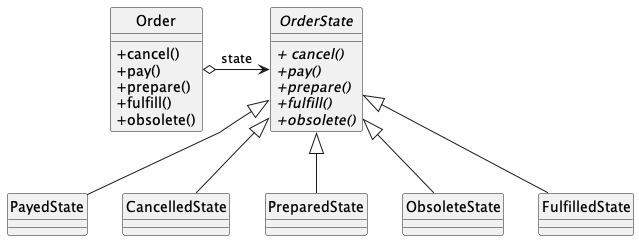
\includegraphics[width=0.8\textwidth]{statePattern}
\centering
\caption{Diagramme de Classe d'étude préliminaire d'implémentation du patron de conception State}
\label{uml:state}
\end{figure}

\paragraph{State: } pour la gestion du statut de commande, nous avons étudier 
l'implémentation du patron de conception State. Ce patron de conception semblait approprié car
il aurait permit de modifier les actions des méthodes en fonction du statut de la commande. Par exemple
nous aurions pu empêcher l'annulation de la commande à partir du moment ou la commande est en cours de préparation.
Cependant, nous avons choisi de ne pas implémenter ce patron de conception car nous avions déjà implémenté 
toutes les fonctionnalités sur la gestion des status des commandes.
